\documentclass{elsarticle}
\usepackage[a4paper, left=3.5cm, right=3.5cm, top=2.5cm, bottom=2.5cm]{geometry}
\usepackage{graphicx}
\usepackage[utf8]{inputenc}
\usepackage{epstopdf}
\usepackage{subfigure}
\usepackage{amsmath}
\usepackage{float}
\usepackage{lineno,hyperref}
\usepackage{url}
%\modulolinenumbers[5]

\pdfstringdefDisableCommands{%
  \def\log{}%
  \def\sum{}%
  \def\rightarrow{}%
}

\journal{Journal of \LaTeX Templates}

%%%%%%%%%%%%%%%%%%%%%%%
%% Elsevier bibliography styles
%%%%%%%%%%%%%%%%%%%%%%%
%% To change the style, put a % in front of the second line of the current style and
%% remove the % from the second line of the style you would like to use.
%%%%%%%%%%%%%%%%%%%%%%%

%% Numbered
%\bibliographystyle{model1-num-names}

%% Numbered without titles
%\bibliographystyle{model1a-num-names}

%% Harvard
%\bibliographystyle{model2-names.bst}\biboptions{authoryear}

%% Vancouver numbered
%\usepackage{numcompress}\bibliographystyle{model3-num-names}

%% Vancouver name/year
%\usepackage{numcompress}\bibliographystyle{model4-names}\biboptions{authoryear}

%% APA style
\bibliographystyle{model5-names}\biboptions{authoryear}

%% AMA style
%\usepackage{numcompress}\bibliographystyle{model6-num-names}

%% `Elsevier LaTeX' style
% \bibliographystyle{elsarticle-num}
%%%%%%%%%%%%%%%%%%%%%%%

\begin{document}

\begin{frontmatter}

\title{Analysis of the high-frequency volume-price relationship of Bitcoin}
%\tnoteref{mytitlenote}}
%\tnotetext[mytitlenote]{Fully documented templates are available in the elsarticle package on \href{http://www.ctan.org/tex-archive/macros/latex/contrib/elsarticle}{CTAN}.}

%% Group authors per affiliation:
%\author{Elsevier\fnref{myfootnote}}
%\address{Radarweg 29, Amsterdam}
%\fntext[myfootnote]{Since 1880.}
\author[mymainaddress]{Fang Wan}

% or include affiliations in footnotes:
\author[mymainaddress,mysecondaryaddress]{Chun-Xiao Nie\corref{mycorrespondingauthor}}
\cortext[mycorrespondingauthor]{Corresponding author}
\ead{niechunxiao2009@163.com; niechunxiao@zjgsu.edu.cn}


%\author[mymainaddress]{Haoxuan Ma\fnref{myfootnote}}
%\fntext[myfootnote]{18767998418@163.com}

\address[mymainaddress]{School of Statistics and Mathematics, Zhejiang Gongshang University, Hangzhou 310018, China}
\address[mysecondaryaddress]{Collaborative Innovation Center of Statistical Data Engineering, Technology \& Application, Zhejiang Gongshang University, Hangzhou, 310018, China}

\begin{abstract}

\end{abstract}

\begin{keyword}
Information flow  \sep Transfer entropy \sep Cryptocurrency market \sep Volume-price relationship
%\JEL C32 \sep  C58 \sep G14
\end{keyword}

\end{frontmatter}
%
\linenumbers

\section{Introduction}
Research into the volume-price relationship provides insights into the underlying mechanisms of market efficiency and liquidity formation. By quantifying the extent to which volume influences or predicts price, analysts can develop more robust models for risk management, trading strategies, and regulatory assessments.

\section{Data and Software}
The primary data source used in this study is the Gemini Exchange dataset available from \texttt{https://www.cryptodatadownload.com/data/gemini/}, which provides minute-level historical data from 2017 through the most recently available period for Bitcoin trading. This dataset includes timestamped open, high, low, close (OHLC) prices, and trading volume calculated in BTC and USD. The high-frequency nature of the data enables fine-grained temporal analysis and makes it particularly suitable for exploring information flow dynamics within short time intervals. The software implemented in our analysis is R with several well-verified packages mentioned in Section \ref{sec:method}. The general view of our data is shown as below. We consider only days with over 90\% minute-level data available for the analysis, and the valid days for each year are shown in Table \ref{tab01_valid_days}. The summary statistics of the high-frequency close price and trading volume are shown in Table \ref{tab:price_stats} and Table \ref{tab:volume_stats} respectively. The data is then transformed into two log returns, and are denoted as $r^{(P)}$ and $r^{(V)}$ for price and volume respectively.


\begin{table}[H]
  \caption{Valid Days for Each Year in the Dataset}
  \label{tab01_valid_days}
  \centering
  \begin{tabular}{lc}
    \hline\noalign{\smallskip}
    \textbf{Year} & \textbf{Valid Days} \\
    \hline\noalign{\smallskip}
    2017 & 111 \\
    2018 & 94 \\
    2019 & 49 \\
    2020 & 195 \\
    2021 & 359 \\
    2022 & 314 \\
    2023 & 30 \\
    2024 & 140 \\
    2025 & 65 \\
    \hline
  \end{tabular}
\end{table}

\begin{table}[H]
  \caption{Summary statistics of the high-frequency Close Price(calculated in USD)}
  \label{tab:price_stats}
  \centering
  \begin{tabular}{lrrrr}
    \hline\noalign{\smallskip}
    \textbf{Year} & \textbf{Mean} & \textbf{Std} & \textbf{Skewness} & \textbf{Kurtosis} \\
    \hline\noalign{\smallskip}
    2017 & 7323.06  & 4905.62  & 0.9181   & -0.4115  \\
    2018 & 9681.76  & 2826.69  & 0.1143   & 0.0823   \\
    2019 & 9205.53  & 1968.58  & -0.2179  & -0.4777  \\
    2020 & 12762.69 & 5245.04  & 0.9788   & 0.4220   \\
    2021 & 47424.68 & 9802.02  & -0.0576  & -1.1365  \\
    2022 & 29678.15 & 10009.00 & 0.2697   & -1.5421  \\
    2023 & 29687.64 & 7180.20  & 0.7205   & -0.5403  \\
    2024 & 75431.92 & 17850.48 & 0.0627   & -1.1986  \\
    2025 & 94123.43 & 7461.64  & -0.2667  & -1.0735  \\
    \hline
  \end{tabular}
\end{table}

\begin{table}[H]
  \caption{Summary statistics of the high-frequency Trading Volume(calculated in BTC)}
  \label{tab:volume_stats}
  \centering
  \begin{tabular}{lrrrr}
    \hline\noalign{\smallskip}
    \textbf{Year} & \textbf{Mean} & \textbf{Std} & \textbf{Skewness} & \textbf{Kurtosis} \\
    \hline\noalign{\smallskip}
    2017 & 8.96  & 28.97  & 34.32  & 2278.52 \\
    2018 & 6.10  & 13.52  & 10.60  & 259.67 \\
    2019 & 3.18  & 12.65  & 13.87  & 340.38 \\
    2020 & 2.04  & 7.71   & 16.00  & 463.17 \\
    2021 & 1.52  & 4.95   & 26.14  & 1770.81 \\
    2022 & 1.06  & 4.48   & 25.13  & 1253.53 \\
    2023 & 0.58  & 2.17   & 25.10  & 1381.38 \\
    2024 & 0.84  & 1.85   & 8.88   & 194.07 \\
    2025 & 0.78  & 1.64   & 7.94   & 143.46 \\
    \hline
  \end{tabular}
\end{table}
It is obivious that the price grows rapidly from 2017 to 2025, with the its distribution much level than normal, and slightly positive skewness. From the perspective of volume, the distribution is hight skewed and heavy-tailed, with the mean volume decreasing from 2017 to 2025. This indicates that in this fast, extensive market, the growth of trading scale of Bitcoin is imbalance with the increase of its price, which implies a non-linear relationship can be captured.

\section{Method}\label{sec:method}
\subsection{Transfer entropy({TE}) with Markov Block Bootstrap}
Transfer entropy is used to capture the non-linear and directional information flow between time series, with that from $X = \{x_{t}\}$ to $Y = \{y_{t}\}$ defined as Eq. \ref{eq01} \cite{TE01}.
\begin{equation} \label{eq01}
  TE_{y \rightarrow x} = \sum p(x_{t+1}, \mathbf{x}_t^{(k)}, \mathbf{y}_t^{(l)}) \log \frac{p(x_{t+1} \mid \mathbf{x}_t^{(k)}, \mathbf{y}_t^{(l)})}{p(x_{t+1} \mid \mathbf{x}_t^{(k)})}
  \end{equation}
  where $\mathbf{x}_t^{(k)} = (x_{t-k+1}, \dots, x_t)$ and $\mathbf{y}_t^{(l)} = (y_{t-l+1}, \dots, y_t)$ denote the k-lag and l-lag historical state vectors of $x$ and $y$ respectively, with the number of states is determined as 4 by quantiles as Eq. \ref{eq02}. Besides, a 600-time Markov Block Bootstrap is adopted to preserve the local dynamics between the series while eliminating the global dependency, the significance of the true $TE$ is obtained from the surrogate distribution of the generated $TE$s, where the smaller the $p$-value, the more significant the information flow.

\begin{equation}\label{eq02}
x^{'}_{t}=\left\{
\begin{array}{rcl}
s_{1}       & & {x_{t} \leq q_{0.1}}\\
s_{2}       & & {x_{t} \in (q_{0.1},q_{0.5}] }\\
s_{3}       & & {x_{t} \in (q_{0.5},q_{0.9}] }\\
s_{4}       & & {x_{t} > q_{0.9}} \\
\end{array} \right.
\end{equation}

\subsection{VAR-based TE analysis}
Given that VAR models are widely used to capture linear interdependencies, which can be expressed as Eq. \ref{eq03}:
\begin{equation} \label{eq03}
    \begin{bmatrix}
    r_t^{(P)} \\
    r_t^{(V)}
    \end{bmatrix}
    =
    c + \sum_{i=1}^{3} A_i
    \begin{bmatrix}
    r_{t-i}^{(P)} \\
    r_{t-i}^{(V)}
    \end{bmatrix}
    + \epsilon_t
    \end{equation}

  Here, $A_i$ represents the coefficient matrices capturing linear dependencies at lag $i$ , and $\epsilon_t$ is a 2-dimensional residual vector, isolating the nonlinear parts of the $r^{(P)}$ and $r^{(V)}$ that cannot be explained by VAR. With the significance evaluated by the combination of JB test, Ljung-Box test and ARCH LM test, where smaller $p$-values for the JB and LM tests indicate better results, and larger $p$-values for the LB test indicate better results.
  
  To analyze nonlinear components individually in the volume-price relationship, we design a implementation based on transfer entropy (TE) and vector autoregression (VAR):
\begin{itemize}
  \item[1.] Firstly, we compute the transfer entropy (TE) bidirectionally between $r^{(P)}$ and $r^{(V)}$, with the result denoted as $TE_{p\rightarrow v}$ and $TE_{v\rightarrow p}$. Based on these TE results, we put analysis on the directional dominance and higher moments of TE.
  \item[2.] Secondly, we fit a VAR with order up to 3 between $r^{(P)}$ and $r^{(V)}$, and evaluating the significance of VAR with a combination of JB test(Eq. \ref{eq04}), Ljung-Box test(Eq. \ref{eq05}) and ARCH LM test(Eq. \ref{eq06}) on each residual respectively, and a primal idea towards the different components in the price-volume relationship will be obtained from the result.
  % JB test
  \begin{equation} \label{eq04}
    JB = \frac{n}{6} \left( S^2 + \frac{(K - 3)^2}{4} \right)
  \end{equation}
  % LB test
  \begin{equation} \label{eq05}
    Q = n(n+2) \sum_{k=1}^{h} \frac{\hat{\rho}_k^2}{n - k}
  \end{equation}
% LM test
  \begin{equation} \label{eq06}
    LM = n(n+2) \sum_{k=1}^{h} \frac{\hat{\rho}_k^2}{n - k}
  \end{equation}

  In these equations, $S$, $K$, $n$, $h$, and \(\hat{\rho}_k\) denote skewness, kurtosis, length of the residual observed, lag order, and autocorrelation at lag $k$, respectively. The significance of the residuals is assessed via the Jarque-Bera (JB) test for normality and the Ljung-Box (Q) test for autocorrelation. The corresponding $p$-values are computed under the null hypotheses of normality ($\chi^2_2$ distribution) and white noise ($\chi^2_h$ distribution), respectively.
  \item[3.] We then recompute bidirectional TE on the residuals to measure the information flow of the nonlinear components.By comparing TE before and after filtering, we can model the relative strength of linear and nonlinear causality and distinguish their respective roles in market dynamics. 

\end{itemize}
\subsection{Mann-Kendall Trend}
To further evaluate trend inside the TE calculated, we applied the Mann-Kendall (MK) test to the daily TE series, The definition of the MK test contains two parts as Eq. \ref{eq06} and Eq. \ref{eq07}, where the satistics $Z$ itself represent both the direction and the significance of the trend, for $Z$ rising to 1 represent a significant upward trend, and falling to -1 represent a significant downward trend.

\begin{equation} \label{eq07}
S = \sum_{i=1}^{n-1} \sum_{j=i+1}^{n} \text{sign}(x_j - x_i)
\end{equation}

\begin{equation} \label{eq08}
Z = 
\begin{cases}
\frac{S - 1}{\sqrt{\text{Var}(S)}} & \text{if } S > 0 \\
0 & \text{if } S = 0 \\
\frac{S + 1}{\sqrt{\text{Var}(S)}} & \text{if } S < 0
\end{cases}
\end{equation}
\section{Results}
\subsection{Volume-price relationship of high-frequency data}
Based on the transfer entropy (TE) calculated for each day, we compute Annual Summaries of TE for both direction, which are offered in Tab. \ref{tab:te_p2v_stats} and Tab. \ref{tab:te_v2p_stats}. hype skewness and kurtosis are observed in 2017, 2021, 2022 and 2025, showing that the price-volume relation tend to get more significant when the market is in drastic volatility. By comparing the $\bar{p}$ of TE betwen the two direction, the one from price to volume is much lower, which means the information flow from price to volume is more significant, indicating the market is generally driven more by price than volume, however, On the TE value it self, We found the average of $TE_{v \rightarrow p}$ is slightly higher than $TE_{p \rightarrow v}$, which indicates that though the information flow from volume to price is less significant, a stable part of non-linear information flow from volume to price is coverd by the the dominant bidirectional linear one.(Details in Sec. \ref{sec:var}).
% --------- PATCHED TABLE: P -> V -----------
\begin{table}[H]
  \caption{Moments \& Significance of TE from Price to Volume ($TE_{P \rightarrow V}$)}
  \label{tab:te_p2v_stats}
  \centering
  \begin{tabular}{crrrrc}
    \hline\noalign{\smallskip}
    \textbf{Year} & \textbf{Mean} & \textbf{Std} & \textbf{Skewness} & \textbf{Kurtosis} & \textbf{$\bar{p}$} \\
    \hline\noalign{\smallskip}
    2017 & 0.0226 & 0.0052 & 0.2346 & 0.0073 & 0.1234 \\
    2018 & 0.0238 & 0.0111 & \textbf{5.0787} & \textbf{32.0705} & 0.1284 \\
    2019 & 0.0229 & 0.0056 & 0.9319 & 0.7630 & 0.2129 \\
    2020 & 0.0220 & 0.0054 & 0.5658 & 0.1045 & 0.2020 \\
    2021 & 0.0212 & 0.0251 & \textbf{17.8038} & \textbf{330.1464} & 0.2575 \\
    2022 & 0.0238 & 0.0267 & \textbf{11.8465} & \textbf{145.9301} & 0.2354 \\
    2023 & 0.1545 & 0.2303 & 1.2866 & -0.1367 & 0.2873 \\
    2024 & 0.0920 & 0.1670 & 2.1809 & 3.2453 & 0.2624 \\
    2025 & 0.0373 & 0.0785 & \textbf{5.7141} & \textbf{32.5258} & 0.2614 \\
    \hline
  \end{tabular}
\end{table}

% --------- PATCHED TABLE: V -> P -----------
\begin{table}[H]
  \caption{Moments \& Significance of TE from Volume to Price ($TE_{V \rightarrow P}$)}
  \label{tab:te_v2p_stats}
  \centering
  \begin{tabular}{crrrrc}
    \hline\noalign{\smallskip}
    \textbf{Year} & \textbf{Mean} & \textbf{Std} & \textbf{Skewness} & \textbf{Kurtosis} & \textbf{$\bar{p}$} \\
    \hline\noalign{\smallskip}
    2017 & 0.0284 & 0.0066 & 0.6172 & -0.0201 & 0.3550 \\
    2018 & 0.0299 & 0.0154 & \textbf{6.8460} & \textbf{57.5926} & 0.3710 \\
    2019 & 0.0257 & 0.0061 & 0.0381 & -0.2896 & 0.3893 \\
    2020 & 0.0257 & 0.0066 & 0.4806 & -0.0247 & 0.4033 \\
    2021 & 0.0243 & 0.0188 & \textbf{16.3237} & \textbf{293.5880} & 0.4673 \\
    2022 & 0.0259 & 0.0174 & \textbf{10.6488} & \textbf{134.4553} & 0.3987 \\
    2023 & 0.1433 & 0.2221 & 1.7369 & 2.1892 & 0.3688 \\
    2024 & 0.0911 & 0.1634 & 2.3158 & 4.2528 & 0.3461 \\
    2025 & 0.0397 & 0.0888 & \textbf{5.5911} & \textbf{30.6203} & 0.3084 \\
    \hline
  \end{tabular}
\end{table}
Consequently, we did another comparison over the TE value pairly in a day, with the results shown in fig \ref{fig:TE_CP_daily}. We found that from a synchronized perspective, the ininformation flow from price to volume is still dominant the price-volume relationship. But the dominance is showing a noticable decreasing trend in recent years, showing a paradiam shift we'd describe in Sec. \ref{sec:var}.

% --------- PATCHED FIGURE: TE CP daily ------
\begin{figure}[H]
  \centering
  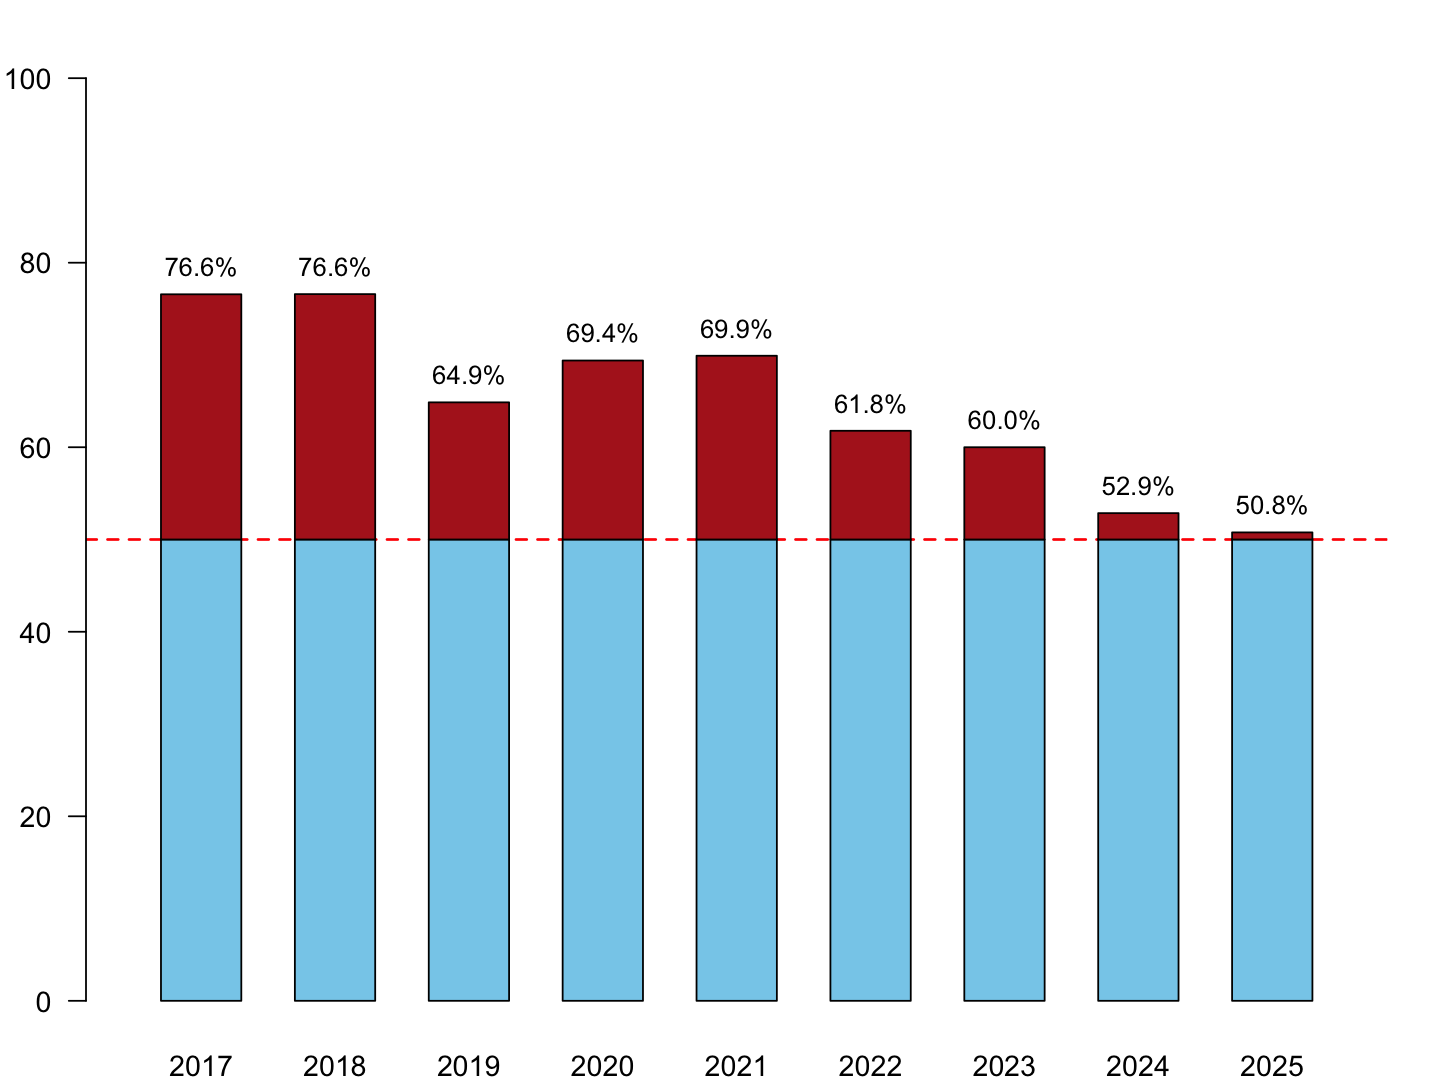
\includegraphics[width=0.75\textwidth]{imgs/greaterRatio.png}
  \caption{Ratio of Days that $TE_{p \rightarrow v}$ > $TE_{v \rightarrow p}$ across years.}
  \label{fig:TE_CP_daily}
  \end{figure}
Besides, we observed specially higher upper quantiles of TE in 2023 and 2024(as shown in Tab. \ref{tab:te_quantiles}), which might be caused by certain market maniputation like The Merge of ETH, and cause the market to form a hyper connection between price and volume.
\begin{table}[H]
  \caption{95\% and 99\% Quantiles of TE from Both Directions}
  \label{tab:te_quantiles}
  \centering
  \begin{tabular}{lllll}
    \hline\noalign{\smallskip}
    \textbf{Year} & $Q_{0.95}^{P \rightarrow V}$ & $Q_{0.99}^{P \rightarrow V}$ & $Q_{0.95}^{V \rightarrow P}$ & $Q_{0.99}^{V \rightarrow P}$ \\
    \hline\noalign{\smallskip}
    2017 & 0.0317 & 0.0339 & 0.0404 & 0.0457 \\
    2018 & 0.0315 & 0.0798 & 0.0435 & 0.0632 \\
    2019 & 0.0339 & 0.0369 & 0.0348 & 0.0388 \\
    2020 & 0.0318 & 0.0358 & 0.0374 & 0.0419 \\
    2021 & 0.0286 & 0.0345 & 0.0340 & 0.0411 \\
    2022 & 0.0314 & 0.0379 & 0.0358 & 0.0465 \\
    2023 & \textbf{0.5931} & \textbf{0.6572} & \textbf{0.5638} & \textbf{0.7595} \\
    2024 & \textbf{0.5195} & \textbf{0.5941} & \textbf{0.4698} & \textbf{0.6575} \\
    2025 & 0.0343 & 0.4505 & 0.0374 & 0.5187 \\
    \hline\noalign{\smallskip}
  \end{tabular}
\end{table}




\subsection{Analysis of VAR filtered volume-price relationships}\label{sec:var}
I this process, we firstly check the results of theVAR itself, with the average lag selected with minium AIC for each day, and $p$-values of JB test, LB test and ARCH LM test shown in Table \ref{tab:var_sig}. The results indicate: 
\begin{itemize}
  \item[1. ] From the period from 2017 to 2020 exhibits strong autocorrelation and significant non-normality in the VAR residuals, reflecting a volatile and structurally complex market.
  \item[2. ] In contrast, from 2021 onward, both the trading volume (Vr) and price (Pr) residuals display diminishing Ljung-Box and ARCH effects, with Jarque-Bera tests suggesting convergence toward normality.
  \item[3. ] This reflects a structural simplification of the market dynamics, with the VAR model capturing most of the linear dependencies — a potential signal of increased market efficiency or post-regime stabilization.
\end{itemize}
Moreover, we observe a consistent asymmetry between the Ljung-Box $p$-values of volume and price residuals, where the residual autocorrelation in trading volume is significantly stronger than that in price across most years, indicating volume series contains more linear conponents that may not be clearly explained by only volume-price relationship. But generally, the results indecating our VAR models are relatively well fitted on these data and non-linear conponents are well extracted, with residuals shown weak non-normality, ARCH effects on both series and autocorrelation at least on $r^{(P)}$.

\begin{table}[H]
  \centering
  \caption{Annual Significance of multi-test in VAR residuals}
  \label{tab:var_sig}
  \begin{tabular}{llllllll}
    \hline\noalign{\smallskip}
    \textbf{Year} & $k_{AIC}$ & $p^{(\mathrm{Vr})}_{\mathrm{JB}}$ & $p^{(\mathrm{Pr})}_{\mathrm{JB}}$ & $p^{(\mathrm{Vr})}_{\mathrm{LB}}$ & $p^{(\mathrm{Pr})}_{\mathrm{LB}}$ & $p^{(\mathrm{Vr})}_{\mathrm{ARCH}}$ & $p^{(\mathrm{Pr})}_{\mathrm{ARCH}}$ \\
    \hline\noalign{\smallskip}
    2017 & 3.000 & \textbf{4.21e-13} & \textbf{0.0000} & \textbf{2.87e-11} & 0.2444 & \textbf{0.0093} & \textbf{0.0070} \\
    2018 & 3.000 & \textbf{1.09e-03} & \textbf{1.35e-04} & \textbf{5.44e-05} & 0.3390 & \textbf{0.0165} & \textbf{0.0220} \\
    2019 & 3.000 & \textbf{6.20e-07} & \textbf{0.0000} & \textbf{5.48e-12} & 0.1455 & \textbf{0.0331} & \textbf{0.0285} \\
    2020 & 3.000 & \textbf{5.08e-04} & \textbf{5.46e-18} & \textbf{2.48e-14} & 0.2462 & \textbf{0.0208} & \textbf{0.0202} \\
    2021 & 2.994 & \textbf{1.99e-03} & \textbf{1.06e-03} & \textbf{1.49e-04} & 0.2556 & \textbf{0.0101} & \textbf{0.0146} \\
    2022 & 2.997 & \textbf{2.20e-03} & \textbf{2.67e-03} & \textbf{1.70e-03} & 0.2427 & \textbf{0.0141} & \textbf{0.0121} \\
    2023 & 2.633 & 1.49e-01 & 1.82e-01 & 1.55e-01 & 0.3418 & 0.1666 & 0.1917 \\
    2024 & 2.771 & 8.15e-02 & 8.91e-02 & 7.30e-02 & 0.2776 & 0.1008 & 0.0895 \\
    2025 & 2.938 & \textbf{1.16e-02} & \textbf{1.05e-02} & \textbf{3.74e-03} & 0.1781 & \textbf{0.0284} & \textbf{0.0297} \\
    \hline
  \end{tabular}
\end{table}

After obtaining the residuals, we recompute the TE on the residuals, It is notable that the $\bar{p}$ of both directions degenerate to the same level, with $\bar{p}$ for $TE_{Pr \rightarrow Vr}$ higher than before(Tab. \ref{tab:te_p2v_stats}) and $\bar{p}$ for $TE_{Vr \rightarrow Pr}$ lower than before(Tab. \ref{tab:te_v2p_stats}), indecating that linear components dominates the information flow from price to volume, while non-linear components dominates the information flow from volume to price. The dynamic remains almost the same on moments of the bidirectional TE, with only few 
\begin{table}[H]
  \caption{Average $p$‑values of $TE$ for Residuals}
  \label{tab:ter_residual_pvalues}
  \centering
  \begin{tabular}{crr}
    \hline\noalign{\smallskip}
    \textbf{Year} & $\bar{p}_{Pr \rightarrow Vr}$ & $\bar{p}_{Vr \rightarrow Pr}$ \\
    \hline\noalign{\smallskip}
    2017 & 0.2522 & 0.1496 \\
    2018 & 0.2552 & 0.3227 \\
    2019 & 0.2436 & 0.2734 \\
    2020 & 0.3914 & 0.3671 \\
    2021 & 0.3795 & 0.4743 \\
    2022 & 0.3619 & 0.4330 \\
    2023 & 0.4007 & 0.4486 \\
    2024 & 0.3118 & 0.3743 \\
    2025 & 0.2276 & 0.3205 \\
    \hline
  \end{tabular}
\end{table}


\begin{table}[H]
  \caption{95\% and 99\% Quantiles of Residual TE from VAR}
  \label{tab:ter_residual_quantiles}
  \centering
  \begin{tabular}{lrrrr}
    \hline\noalign{\smallskip}
    \textbf{Year} & $Q_{0.95}^{Pr \rightarrow Vr}$ & $Q_{0.99}^{Pr \rightarrow Vr}$ & $Q_{0.95}^{Vr \rightarrow Pr}$ & $Q_{0.99}^{Vr \rightarrow Pr}$ \\
    \hline\noalign{\smallskip}
    2017 & 0.0335 & 0.0392 & 0.0869 & 0.1455 \\
    2018 & 0.0373 & 0.0650 & 0.0394 & 0.0585 \\
    2019 & 0.0339 & 0.0372 & 0.0397 & 0.0517 \\
    2020 & 0.0335 & 0.0378 & 0.0325 & 0.0375 \\
    2021 & 0.0310 & 0.0369 & 0.0286 & 0.0331 \\
    2022 & 0.0309 & 0.0428 & 0.0315 & 0.0365 \\
    2023 & 0.5399 & 0.6538 & 0.5670 & 0.6928 \\
    2024 & 0.5471 & 0.6291 & 0.5268 & 0.6531 \\
    2025 & 0.0388 & 0.5075 & 0.0350 & 0.4129 \\
    \hline
  \end{tabular}
\end{table}


\subsection{Trend analysis}
We apply the Mann-Kendall test to the yearly transfer entropy (TE) series to examine directional trends in information flow. The results reveal that TE from price to volume is more likely to show significant changes over time, with a tendency to weaken in recent years, which might be caused by the high value of Bitcoin. In contrast, TE from volume to price, when it shows a trend, is nearly always increasing. This suggests that volume is becoming a stronger leading indicator for price in the cryptocurrency market. Additionally, residual-based TE series uncover asynchronous shifts in information structure, particularly in 2021 and 2022, which may reflect behavioral changes associated with the market's transition from bull to bear conditions.






\section{Conclusions}

\section*{CRediT authorship contribution statement}



\section*{Funding Sources}
The work is supported by the characteristic \& preponderant discipline of key construction universities in Zhejiang province (Zhejiang Gongshang University $-$ Statistics). Fund Number : 1020JYN6523001G-026; 1020JYN6524001G-020



\section*{Declaration of Competing Interest}
The authors declare that they have no known competing financial interests or personal relationships that could have appeared to influence the work reported in this paper. No conflict of interest have been declared by the authors.



\bibliography{mybibfile}
\section*{Appendix}

\begin{table}[H]
  \caption{Moments of $TE_{Pr \rightarrow Vr}$ (Residuals)}
  \label{tab:ter_pr2vr_moments_app}
  \centering
  \begin{tabular}{crrrr}
    \hline\noalign{\smallskip}
    \textbf{Year} & \textbf{Mean} & \textbf{Std} & \textbf{Skewness} & \textbf{Kurtosis} \\
    \hline\noalign{\smallskip}
    2017 & 0.0248 & 0.0054 & 0.4983 & 0.6252 \\
    2018 & 0.0273 & 0.0200 & 8.2555 & 75.2433 \\
    2019 & 0.0258 & 0.0055 & 0.1479 & -0.6447 \\
    2020 & 0.0224 & 0.0060 & 0.8790 & 1.8067 \\
    2021 & 0.0222 & 0.0132 & 13.7429 & 229.5683 \\
    2022 & 0.0243 & 0.0255 & 11.6713 & 141.2074 \\
    2023 & 0.1271 & 0.1917 & 1.7327 & 2.0264 \\
    2024 & 0.0935 & 0.1726 & 2.3455 & 4.1877 \\
    2025 & 0.0407 & 0.0845 & 5.5176 & 29.5499 \\
    \hline
  \end{tabular}
\end{table}

\begin{table}[H]
  \caption{Moments of $TE_{Vr \rightarrow Pr}$ (Residuals)}
  \label{tab:ter_vr2pr_moments_app}
  \centering
  \begin{tabular}{crrrr}
    \hline\noalign{\smallskip}
    \textbf{Year} & \textbf{Mean} & \textbf{Std} & \textbf{Skewness} & \textbf{Kurtosis} \\
    \hline\noalign{\smallskip}
    2017 & 0.0412 & 0.0292 & 2.8593 & 11.8731 \\
    2018 & 0.0256 & 0.0100 & 2.7837 & 11.6623 \\
    2019 & 0.0270 & 0.0090 & 1.0267 & 1.8689 \\
    2020 & 0.0226 & 0.0057 & 0.3192 & 0.1847 \\
    2021 & 0.0205 & 0.0149 & 16.2695 & 292.4390 \\
    2022 & 0.0230 & 0.0238 & 11.6990 & 143.4347 \\
    2023 & 0.1401 & 0.2128 & 1.5154 & 1.0093 \\
    2024 & 0.0933 & 0.1708 & 2.2114 & 3.4608 \\
    2025 & 0.0364 & 0.0755 & 6.0254 & 37.3487 \\
    \hline
  \end{tabular}
\end{table}

\end{document}
